%=======================================================================
% SIPMS - Smart Internship & Project Management System
% Final Project Report (PFE)
% IIT Sfax Template Style
% Author: Ayadi Youssef
% Supervisor: Rahma Bouaziz
% Company: Clinisys
% Date: May 2026
%=======================================================================

%=======================================================================
% Document Class
%=======================================================================
\documentclass[a4paper,12pt,oneside,english]{../IIT_Sfax_Template/Configuration/IIT-report}

%=======================================================================
% Custom Commands
%=======================================================================
\def\reportTitle{Smart Internship \& Project Management System}
\def\reportSubtitle{SIPMS}
\def\name{Ayadi Youssef}
\def\date{May 2026}
\def\supervisor{Rahma Bouaziz}
\def\company{Clinisys}
\def\academicYear{2025-2026}

% Colors
\definecolor{IITBlue}{RGB}{0,126,167}
\definecolor{IITDarkBlue}{RGB}{0,90,120}
\definecolor{PrimaryBlue}{RGB}{0,126,167}

%=======================================================================
% Packages
%=======================================================================
\usepackage{graphicx}
\usepackage{float}
\usepackage{amsmath}
\usepackage{amssymb}
\usepackage{listings}
\usepackage{color}
\usepackage{hyperref}
\usepackage{booktabs}
\usepackage{pgffor}
\usepackage{multicol}

% Code listing style
\definecolor{codegreen}{rgb}{0,0.6,0}
\definecolor{codegray}{rgb}{0.5,0.5,0.5}
\definecolor{codepurple}{rgb}{0.58,0,0.82}
\definecolor{backcolor}{rgb}{0.95,0.95,0.92}

\lstdefinestyle{mystyle}{
    backgroundcolor=\color{backcolor},
    commentstyle=\color{codegreen},
    keywordstyle=\color{blue},
    numberstyle=\tiny\color{codegray},
    stringstyle=\color{codepurple},
    basicstyle=\ttfamily\small,
    frame=single,
    breaklines=true,
}
\lstset{style=mystyle}

%=======================================================================
% Front Matter
%=======================================================================
\begin{document}

%=======================================================================
% Cover Page
%=======================================================================
\thispagestyle{empty}
\begin{center}
\vspace*{1cm}
% University Logo
\begin{figure}[H]
\centering
%
\includegraphics[width=0.25\textwidth]{../IIT_Sfax_Template/images/TemplateImages/IIT-Logo.png}
\end{figure}

\vspace{1cm}
\textbf{\Large INSTITUT INTERNATIONAL DE TECHNOLOGIE}\\[0.3cm]
\textbf{\large IIT - Sfax}\\[2cm]

\textbf{\large Computer Engineering Department}\\[0.5cm]

\vspace{2cm}
\textbf{\LARGE \reportTitle}\\[0.5cm]
\textbf{\large (\reportSubtitle)}\\[2cm]

\textbf{\large \textbf{FINAL PROJECT REPORT (PFE)}}\\[1.5cm]

\begin{minipage}{0.85\linewidth}
\begin{center}
\textbf{Field:} Computer Engineering\\
\textbf{Academic Year:} \academicYear
\end{center}
\end{minipage}

\vspace{2cm}

% Student Info
\begin{tabular}{ll}
\textbf{Student:} & \name \\
\textbf{Supervisor:} & \supervisor \\
\textbf{Company:} & \company \\
\textbf{Date:} & \date
\end{tabular}

\end{center}

\pagebreak

%=======================================================================
% Acknowledgements
%=======================================================================
\thispagestyle{empty}
\chapter*{Acknowledgements}
\addcontentsline{toc}{chapter}{Acknowledgements}

Firstly, I would like to express my sincere gratitude to my supervisor, \textbf{Ms. Rahma Bouaziz}, for her invaluable guidance, continuous support, and constructive feedback throughout this project. Her expertise and encouragement have been instrumental in the successful completion of this work.

I am also grateful to \textbf{Clinisys} for providing me with the opportunity to work on this real-world project and for the valuable industrial experience gained during my internship.

My heartfelt thanks go to my family and friends for their unconditional support and motivation throughout my academic journey.

Finally, I would like to thank all the professors and staff of the Computer Engineering department at IIT for their guidance and knowledge.

\vspace{2cm}
\textbf{May 2026}

%=======================================================================
% Abstract
% ============================================================================
\chapter*{Abstract}
\addcontentsline{toc}{chapter}{Abstract}

This report presents the development of the Smart Internship \& Project Management System (SIPMS), a full-stack web application designed to digitize and automate the internship and academic project management process. The system integrates modern web technologies including React.js for the frontend, Spring Boot for the backend, and MySQL for data persistence. Key features include role-based authentication, automated quiz evaluation with 48-hour time limit, AI-powered project ranking, and intelligent candidate-supervisor matching. The system follows a microservices architecture with JWT-based security and comprehensive audit logging.

\textbf{Keywords:} Internship Management, Web Application, React.js, Spring Boot, AI Integration, Role-Based Access Control, MySQL, JWT Authentication

%=======================================================================
% Table of Contents
%=======================================================================
\dominitoc
\tableofcontents
\pagebreak

%=======================================================================
% List of Figures
%=======================================================================
\listoffigures
\pagebreak

%=======================================================================
% List of Tables
%=======================================================================
\listoftables
\pagebreak

%=======================================================================
% CHAPTER 1: GENERAL INTRODUCTION
% ============================================================================
\chapter{GENERAL INTRODUCTION}

\section{Project Context}
In the current economic context characterized by accelerated digital transformation and increasing competition in the job market, the effective management of internship recruitment processes and academic projects has become a major challenge for organizations. Traditional paper-based manual management methods present numerous limitations: document loss, long processing times, lack of traceability, and inefficiency in evaluating candidate competencies.

The \textbf{Smart Internship \& Project Management System (SIPMS)} is a full-stack web application designed to digitize and automate the entire internship and academic project management process. This system integrates advanced artificial intelligence functionalities for analyzing and ranking projects submitted by candidates, as well as for intelligent matching between candidates and available supervisors.

\begin{figure}[H]
\centering
%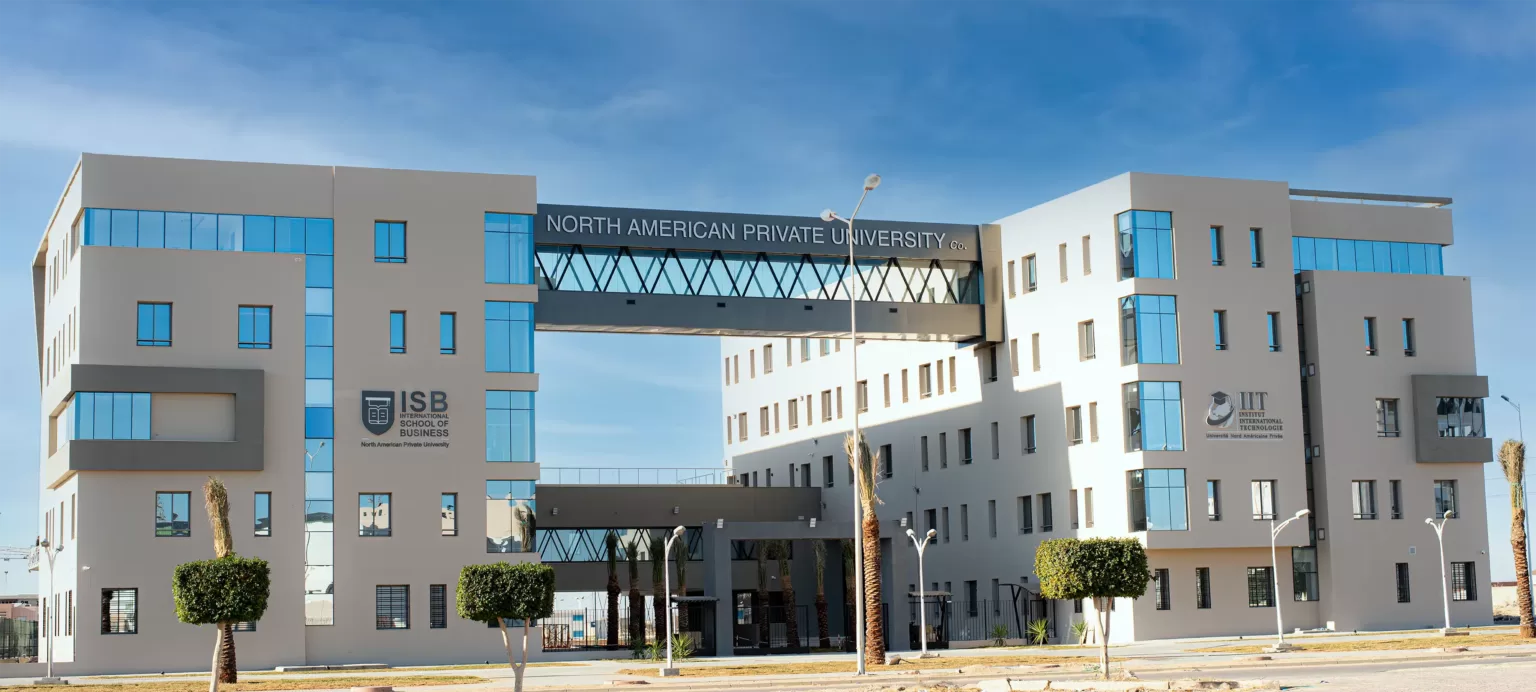
\includegraphics[width=0.8\textwidth]{../IIT_Sfax_Template/images/TemplateImages/Image-Exemple.jpg}
\caption{SIPMS Application Overview}
\end{figure}

\section{Project Objectives}
The main objective of this project is to develop a professional web application that allows:

\begin{enumerate}
    \item \textbf{Digitizing the Application Process}: Enabling candidates to submit their applications online, including their CV and project ideas
    \item \textbf{Automating Evaluation}: Implementing an automated technical quiz system with instant correction to evaluate candidates' technical skills
    \item \textbf{AI Integration}: Using artificial intelligence algorithms to analyze and rank submitted projects, as well as to suggest the most suitable supervisor for each project
    \item \textbf{Role-Based Access Control (RBAC)}: Implementing a role-based access system allowing different user types (Admin, Manager, Receptionist, Candidate) to access appropriate functionalities
    \item \textbf{Automated Notifications}: Triggering automatic in-app and email notifications at each key stage of the selection process
\end{enumerate}

\section{Project Scope}
The SIPMS system covers the following functionalities:

\begin{itemize}
    \item \textbf{Authentication Module}: Secure JWT-based connection with role management
    \item \textbf{Application Management}: Online submission and physical registration
    \item \textbf{Evaluation Module}: Timed technical quiz with automatic correction
    \item \textbf{AI Module}: Project ranking and candidate-supervisor matching
    \item \textbf{Decision Module}: Validation workflow with acceptance/rejection
    \item \textbf{Notification Module}: In-app and email notifications
\end{itemize}

\section{Problem Statement}
Academic organizations and companies face several challenges in internship management:

\begin{table}[H]
\centering
\begin{tabular}{|l|l|}
\hline
\textbf{Identified Problem} & \textbf{SIPMS Solution} \\ \hline
Manual management of physical files & Complete digitization \\ \hline
Long processing times & Process automation \\ \hline
Lack of traceability & Complete audit logs \\ \hline
Subjective evaluation & Standardized quiz + AI \\ \hline
Supervisor/project matching difficulty & Matching algorithm \\ \hline
Inefficient communication & Automated notifications \\ \hline
\end{tabular}
\caption{Problem-Solution Mapping}
\end{table}

\pagebreak

%=======================================================================
% CHAPTER 2: REQUIREMENTS ANALYSIS
% ============================================================================
\chapter{REQUIREMENTS ANALYSIS}

\section{Current Situation Study}
In the traditional internship management system, the process unfolds as follows:

\begin{enumerate}
    \item \textbf{Physical File Reception}: Candidates bring their applications in person to the internship office
    \item \textbf{Manual Filing}: Receptionists sort and file applications
    \item \textbf{Paper Evaluation}: Managers evaluate projects manually
    \item \textbf{Decision by Discussion}: Decisions are made during meetings
    \item \textbf{Communication by Phone/Email}: Candidates are informed individually
\end{enumerate}

\section{Current System Disadvantages}

\begin{itemize}
    \item \textbf{Document Loss}: High risk of loss or misfiling
    \item \textbf{Processing Time}: Average delay of 2-3 weeks
    \item \textbf{Costs}: Storage and personnel expenses
    \item \textbf{No History}: Difficulty consulting old applications
    \item \textbf{Difficult Statistics}: Impossible to generate reports
\end{itemize}

\section{Requirements Analysis}

\subsection{Functional Requirements}

\begin{table}[H]
\centering
\begin{tabular}{|l|c|l|}
\hline
\textbf{Requirement} & \textbf{Priority} & \textbf{Description} \\ \hline
Authentication & High & Secure JWT connection \\ \hline
Candidate Registration & High & Online registration form \\ \hline
Project Submission & High & Submission interface \\ \hline
Technical Quiz & High & Automated evaluation \\ \hline
AI Ranking & Medium & Project analysis \\ \hline
Supervisor Matching & Medium & Supervisor suggestion \\ \hline
Manager Decision & High & Acceptance/Rejection \\ \hline
Notifications & Medium & Automatic emails \\ \hline
User Management & High & CRUD operations \\ \hline
Supervisor Management & High & CRUD operations \\ \hline
Role-Based Redirect & High & Dashboard per role \\ \hline
Password Reset & High & First login change \\ \hline
\end{tabular}
\caption{Functional Requirements}
\end{table}

\subsection{Non-Functional Requirements}

\begin{itemize}
    \item \textbf{Performance}: Response time < 2 seconds
    \item \textbf{Security}: JWT encryption, XSS/SQLi protection
    \item \textbf{Availability}: 99.5\% uptime
    \item \textbf{Scalability}: Modular architecture
    \item \textbf{Maintainability}: Documented code, unit tests
    \item \textbf{User Experience}: Responsive design, Tailwind CSS
\end{itemize}

\section{Business Rules}

\begin{table}[H]
\centering
\begin{tabular}{|l|l|}
\hline
\textbf{Rule ID} & \textbf{Description} \\ \hline
BR-01 & Any physical application must be scanned and associated with a candidate account \\ \hline
BR-02 & A candidate must pass the quiz (≥60\%) before final decision \\ \hline
BR-03 & AI does not make final decisions; it provides a confidence score \\ \hline
BR-04 & A supervisor cannot manage more than 3 interns simultaneously \\ \hline
BR-05 & Every status change triggers an automatic email \\ \hline
BR-06 & Quiz must be completed within 48 hours of assignment \\ \hline
BR-07 & New users must change their temporary password on first login \\ \hline
BR-08 & Each quiz is specific to a specialty (Web, Security, Power BI) \\ \hline
\end{tabular}
\caption{Business Rules}
\end{table}

\pagebreak

%=======================================================================
% CHAPTER 3: TECHNICAL STUDY
% ============================================================================
\chapter{TECHNICAL STUDY}

\section{Technology Choices}

\subsection{Frontend}

\begin{table}[H]
\centering
\begin{tabular}{|l|c|l|}
\hline
\textbf{Tech} & \textbf{Version} & \textbf{Justification} \\ \hline
React & 18.x & Modern framework, large community \\ \hline
Vite & 5.x & Fast build tool \\ \hline
Tailwind CSS & 3.x & Utility-first styling \\ \hline
Axios & 1.x & HTTP client \\ \hline
React Router & 6.x & Client-side routing \\ \hline
Lucide React & Latest & Icon library \\ \hline
\end{tabular}
\caption{Frontend Technologies}
\end{table}

\subsection{Backend}

\begin{table}[H]
\centering
\begin{tabular}{|l|c|l|}
\hline
\textbf{Tech} & \textbf{Version} & \textbf{Justification} \\ \hline
Spring Boot & 3.2.x & Enterprise Java framework \\ \hline
Spring Security & 6.x & Integrated security \\ \hline
JWT & 0.12.x & Stateless authentication \\ \hline
MySQL & 8.0 & Relational database \\ \hline
JPA/Hibernate & 6.x & ORM framework \\ \hline
Java Mail & - & Email notifications \\ \hline
\end{tabular}
\caption{Backend Technologies}
\end{table}

\section{System Architecture}

\begin{figure}[H]
\centering
%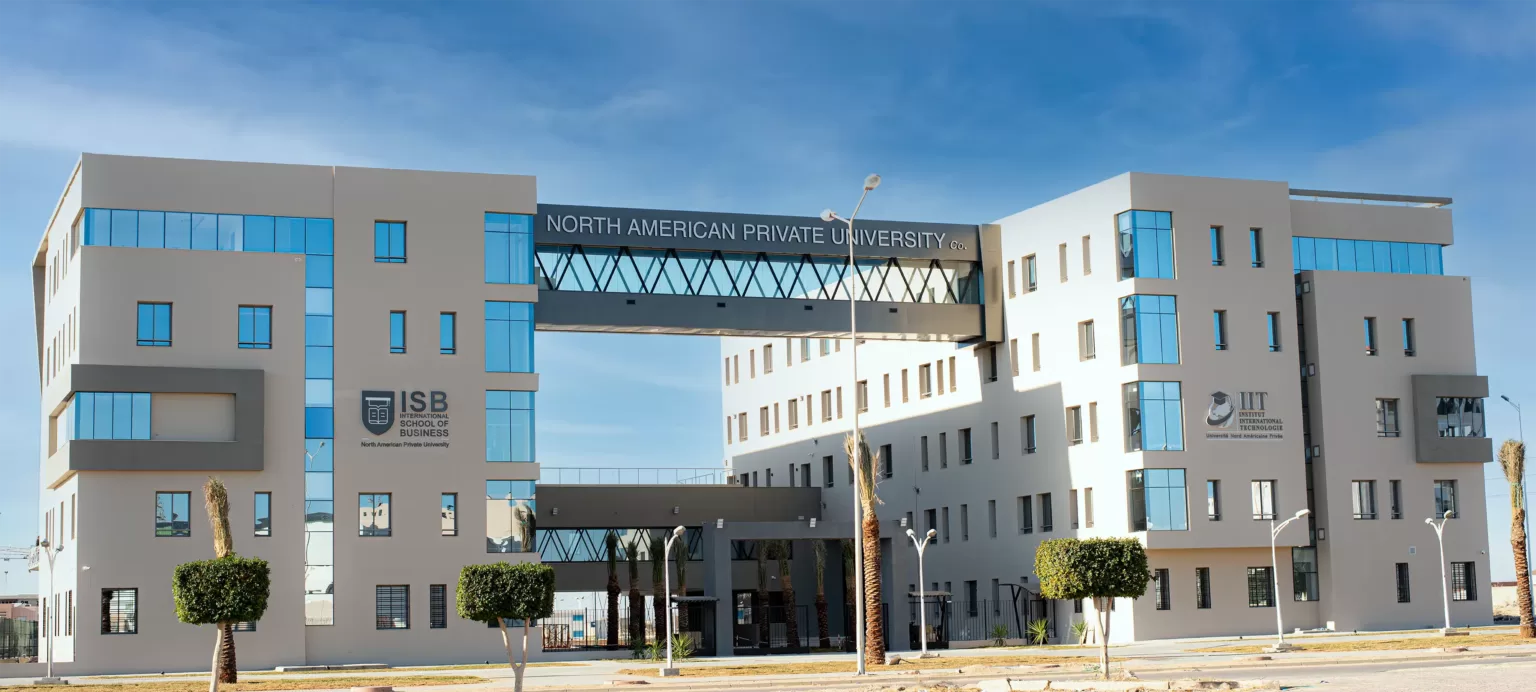
\includegraphics[width=0.9\textwidth]{../IIT_Sfax_Template/images/TemplateImages/Image-Exemple.jpg}
\caption{System Architecture}
\end{figure}

The system follows a three-tier architecture:

\begin{enumerate}
    \item \textbf{Presentation Layer (Frontend)}: React.js with Tailwind CSS running on Vite
    \item \textbf{Application Layer (Backend)}: Spring Boot REST API running on port 8080
    \item \textbf{Data Layer (Database)}: MySQL running on port 3306
\end{enumerate}

\subsection{Architecture Diagram}

\begin{figure}[H]
\centering
\begin{tabular}{|c|}
\hline
\Client (React - Port 5173) \\
\hline
$\downarrow$ \\
\hline
\Vite Proxy \\
\hline
$\downarrow$ \\
\hline
\Spring Boot API (Port 8080) \\
\hline
$\downarrow$ \\
\hline
\MySQL Database (Port 3306) \\
\hline
\end{tabular}
\caption{Architecture Layers}
\end{figure}

\pagebreak

\section{UML Diagrams}

\subsection{Use Case Diagram}

\begin{figure}[H]
%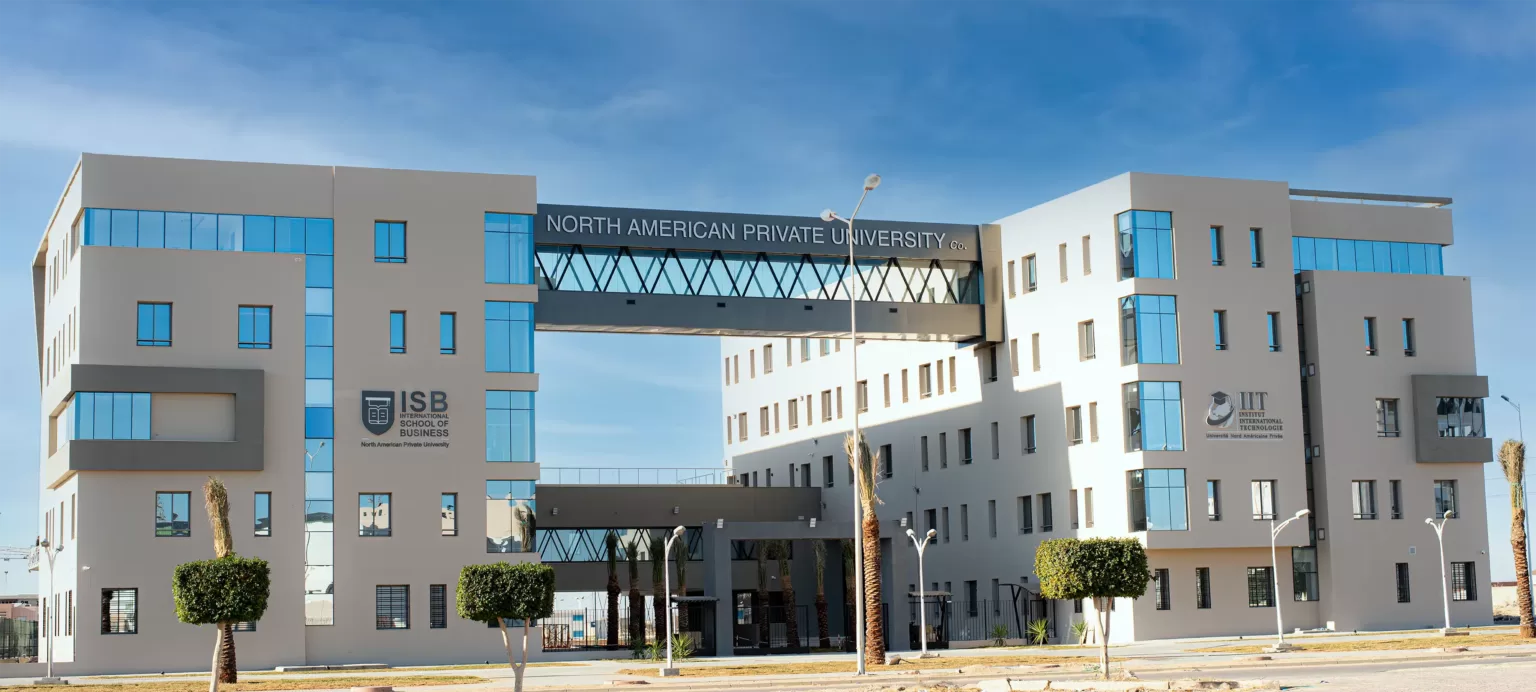
\includegraphics[width=0.9\textwidth]{../IIT_Sfax_Template/images/TemplateImages/Image-Exemple.jpg}
\caption{Use Case Diagram - SIPMS}
\end{figure}

Actors in the system:

\begin{enumerate}
    \item \textbf{Admin}: System administration, user management
    \item \textbf{Manager}: Review applications, make decisions, assign supervisors
    \item \textbf{Receptionist}: Register physical dossiers, manage candidates
    \item \textbf{Candidate}: Submit applications, take quizzes, view results
\end{enumerate}

Use Cases:

\begin{itemize}
    \item Authentication (Login/Logout)
    \item User Management (CRUD)
    \item Supervisor Management (CRUD)
    \item Application Submission
    \item Quiz Taking
    \item AI Analysis
    \item Notifications
\end{itemize}

\subsection{Class Diagram (Key Entities)}

\begin{figure}[H]
%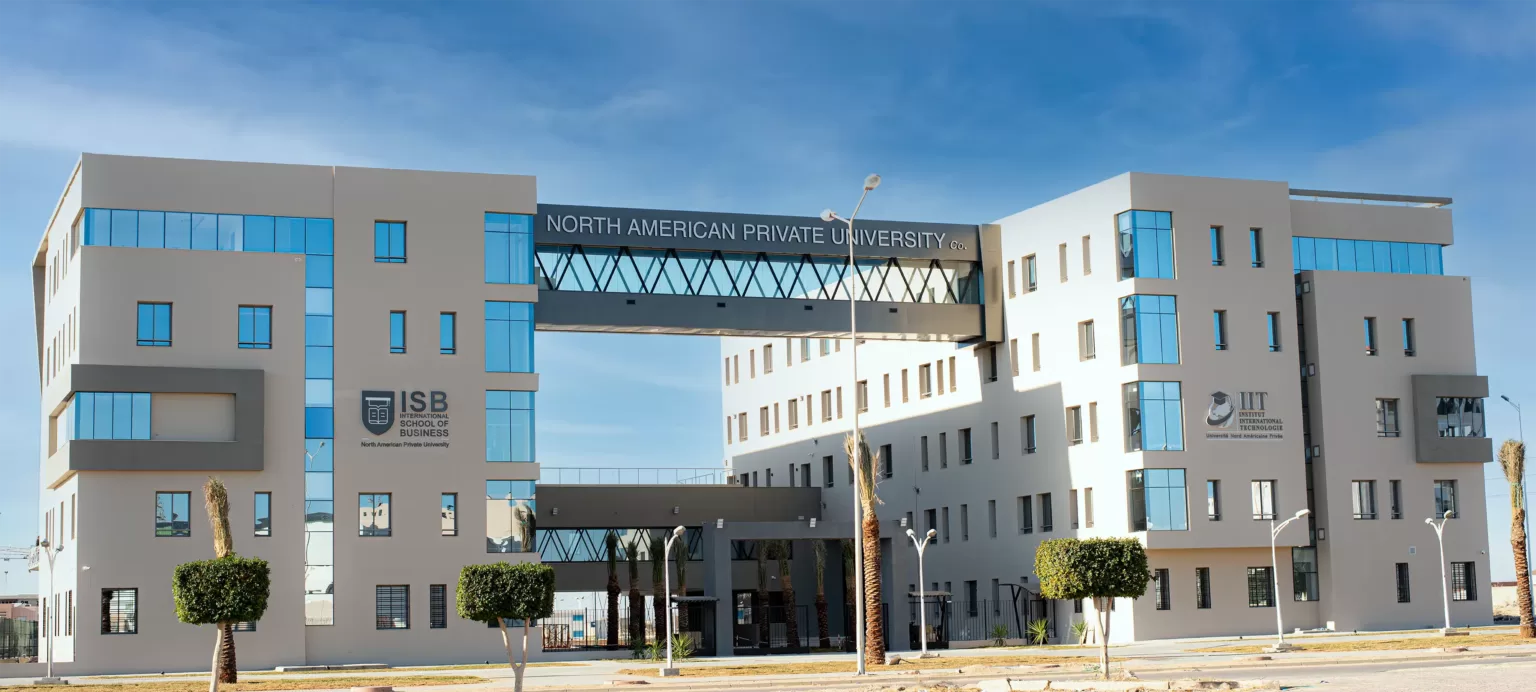
\includegraphics[width=0.9\textwidth]{../IIT_Sfax_Template/images/TemplateImages/Image-Exemple.jpg}
\caption{Class Diagram - Main Entities}
\end{figure}

Key Entities:
\begin{itemize}
    \item \textbf{User}: Base authentication entity with roles
    \item \textbf{Candidate}: Extended user profile with specialty
    \item \textbf{Supervisor}: Project mentor with capacity
    \item \textbf{Project}: Internship project idea
    \item \textbf{Application}: Main lifecycle entity
    \item \textbf{Quiz}: Assessment with questions
    \item \textbf{QuizAttempt}: Candidate quiz submission
    \item \textbf{Notification}: System alerts
\end{itemize}

\pagebreak

\subsection{Sequence Diagrams}

%\subsubsection*{Authentication Flow}

\begin{figure}[H]
%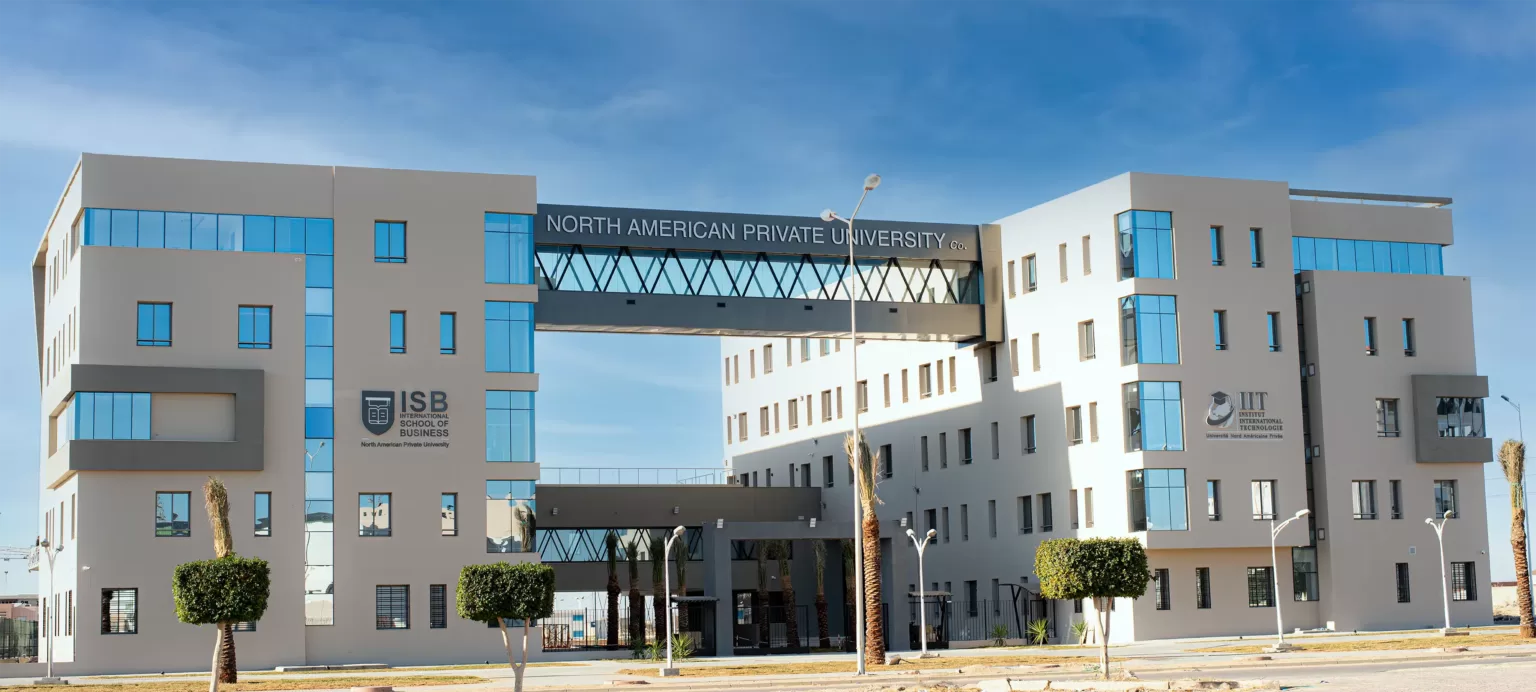
\includegraphics[width=0.9\textwidth]{../IIT_Sfax_Template/images/TemplateImages/Image-Exemple.jpg}
\caption{Sequence Diagram - Authentication}
\end{figure}

Login Flow:
\begin{enumerate}
    \item User enters credentials
    \item Frontend calls auth API
    \item Backend validates and returns JWT
    \item Frontend stores token in localStorage
    \item AuthContext updates state
    \item useEffect redirects based on role
\end{enumerate}

%\subsubsection*{Quiz Flow}

\begin{figure}[H]
%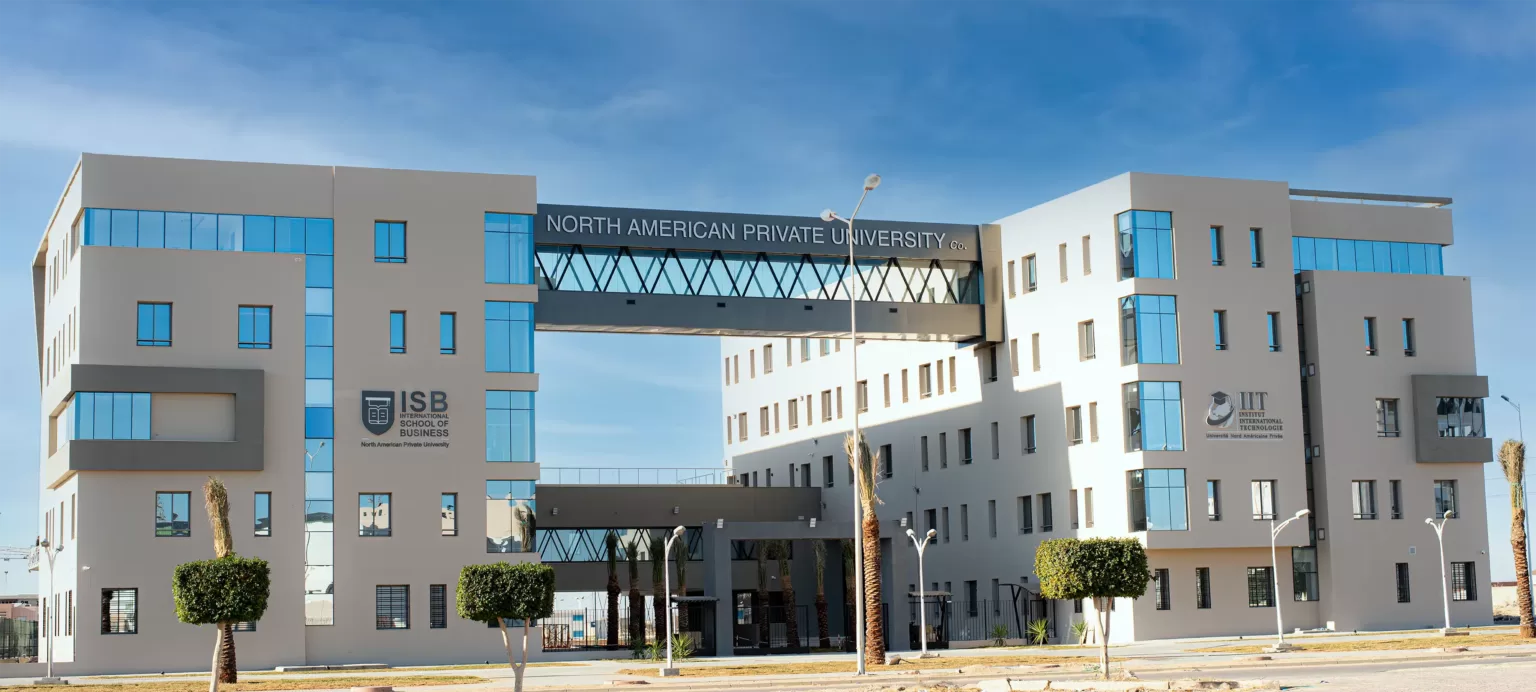
\includegraphics[width=0.9\textwidth]{../IIT_Sfax_Template/images/TemplateImages/Image-Exemple.jpg}
\caption{Sequence Diagram - Quiz Submission}
\end{figure}

Quiz Flow:
\begin{enumerate}
    \item Candidate starts quiz
    \item System creates QuizAttempt with 48h expiry
    \item Candidate answers questions
    \item System auto-grades on submission
    \item Score calculated and saved
    \item Candidate status updated
\end{enumerate}

\pagebreak

%=======================================================================
% CHAPTER 4: IMPLEMENTATION
% ============================================================================
\chapter{IMPLEMENTATION}

\section{Project Structure}

\begin{figure}[H]
%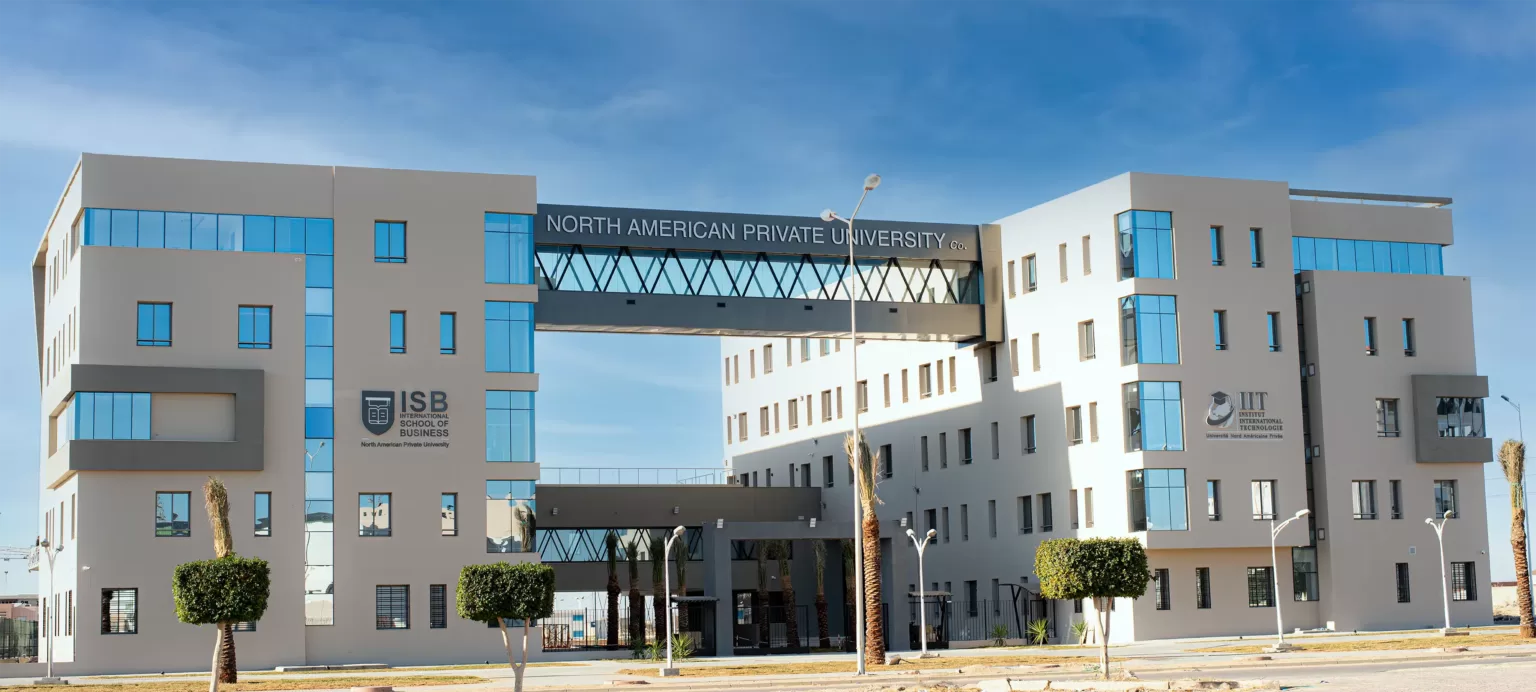
\includegraphics[width=0.9\textwidth]{../IIT_Sfax_Template/images/TemplateImages/Image-Exemple.jpg}
\caption{Project Structure}
\end{figure}

\begin{verbatim}
SIPMS/
├── backend/                    # Spring Boot API
│   ├── src/main/java/com/project/sipms/
│   │   ├── controller/       # REST APIs
│   │   ├── service/         # Business logic
│   │   ├── repository/      # Data access
│   │   ├── entity/          # JPA entities
│   │   ├── dto/             # Data transfer objects
│   │   ├── security/        # JWT & auth
│   │   ├── ai/              # AI algorithms
│   │   └── common/          # Utilities
│   └── src/main/resources/
│       └── application.properties
│
├── frontend/                  # React Application
│   ├── src/
│   │   ├── pages/            # Dashboard pages
│   │   ├── components/       # Reusable components
│   │   ├── api/              # Axios config
│   │   ├── context/          # React contexts
│   │   └── layouts/          # Layout components
│   └── package.json
│
└── docs/                     # Documentation
\end{verbatim}

\section{Development Phases}

\subsection{Phase 1: Configuration (Week 1-2)}
\begin{itemize}
    \item Spring Boot project setup with dependencies
    \item React + Vite + Tailwind setup
    \item MySQL and JPA configuration
    \item JWT authentication setup
\end{itemize}

\subsection{Phase 2: Authentication (Week 3)}
\begin{itemize}
    \item Login/Logout with JWT
    \item Role-based access control
    \item Password reset on first login
    \item Demo mode for testing
\end{itemize}

\subsection{Phase 3: User Management (Week 4)}
\begin{itemize}
    \item User CRUD operations
    \item Auto-generated passwords
    \item Email notifications
    \item Demo mode with localStorage
\end{itemize}

\subsection{Phase 4: Supervisor Management (Week 5)}
\begin{itemize}
    \item Supervisor CRUD
    \item Capacity tracking
    \item Expertise tags
\end{itemize}

\subsection{Phase 5: Application Module (Week 6-7)}
\begin{itemize}
    \item Online submission
    \item Physical registration
    \item Status management
    \item AI score integration
\end{itemize}

\subsection{Phase 6: Quiz System (Week 8)}
\begin{itemize}
    \item Quiz with 48-hour timer
    \item Auto-correction
    \item Score calculation
    \item Specialty-based quizzes
\end{itemize}

\pagebreak

\section{Backend Implementation}

\subsection{User Entity}
\begin{lstlisting}[language=Java, caption=User Entity]
@Entity
@Table(name = "users")
public class User {
    @Id @GeneratedValue
    private Long id;
    
    private String firstName;
    private String lastName;
    private String email;
    private String passwordHash;
    private boolean active;
    private boolean mustChangePassword;
    
    @ManyToMany
    @JoinTable(name = "user_roles")
    private Set<Role> roles;
    
    private LocalDateTime createdAt;
    private LocalDateTime updatedAt;
}
\end{lstlisting}

%\subsection{Auth Controller}
\begin{lstlisting}[language=Java, caption=Auth Controller]
@RestController
@RequestMapping("/api/auth")
public class AuthController {
    
    @PostMapping("/login")
    public ResponseEntity<ApiResponse<AuthResponse>> login(
            @RequestBody LoginRequest request) {
        // Validate credentials
        // Generate JWT token
        // Return user info with roles
    }
}
\end{lstlisting}

%\subsection{Quiz Service}
\begin{lstlisting}[language=Java, caption=Quiz Service]
@Service
public class QuizService {
    
    public QuizResultDto submitQuiz(QuizSubmissionRequest request) {
        // Calculate score
        // Save attempt
        // Update candidate status
        // Return results
    }
}
\end{lstlisting}

\pagebreak

\section{Frontend Implementation}

%\subsection{Auth Context}
\begin{lstlisting}[language=JavaScript, caption=Auth Context (React)]
const authReducer = (state, action) => {
    switch (action.type) {
        case 'LOGIN':
            return {
                ...state,
                user: action.payload.user,
                token: action.payload.token,
                isAuthenticated: true,
                isLoading: false,
            };
        case 'LOGOUT':
            // Nuclear logout - clear everything
            localStorage.removeItem('sipms_token');
            localStorage.removeItem('sipms_user');
            sessionStorage.clear();
            return { ...initialState, isLoading: false };
        default:
            return state;
    }
};
\end{lstlisting}

%\subsection{Login with Role-Based Redirect}
\begin{lstlisting}[language=JavaScript, caption=Login Page - Role-Based Redirect]
export default function LoginPage() {
    const { login, isAuthenticated } = useAuth();
    const navigate = useNavigate();
    const loginSuccessRef = useRef(false);

    useEffect(() => {
        if (isAuthenticated && loginSuccessRef.current) {
            loginSuccessRef.current = false;
            const user = JSON.parse(localStorage.getItem('sipms_user'));
            
            if (user.mustChangePassword) {
                navigate('/reset-password');
            } else if (user.roles.includes('ROLE_RECEPTIONIST')) {
                navigate('/reception-panel');
            } else if (user.roles.includes('ROLE_CANDIDATE')) {
                navigate('/quiz-interface');
            } else {
                navigate('/dashboard');
            }
        }
    }, [isAuthenticated]);
}
\end{lstlisting}

%\subsection{User Creation with Auto-Generated Password}
\begin{lstlisting}[language=JavaScript, caption=User Creation]
const handleSaveAdd = async () => {
    // Auto-generate secure password
    const tempPassword = generateSecurePassword();
    const userData = { 
        ...formData, 
        password: tempPassword, 
        mustChangePassword: true 
    };
    
    await usersApi.create(userData);
    
    alert(`User created!\nEmail: ${email}\nPassword: ${tempPassword}`);
};
\end{lstlisting}

\pagebreak

%=======================================================================
% CHAPTER 5: USER INTERFACE
% ============================================================================
\chapter{USER INTERFACE}

\section{Design System}

\subsection{Color Palette}

\begin{table}[H]
\centering
\begin{tabular}{|l|c|l|}
\hline
\textbf{Color} & \textbf{Hex Code} & \textbf{Usage} \\ \hline
Primary & \#007EA7 & Primary buttons, links \\ \hline
Primary Light & \#00A8E8 & Hover states \\ \hline
Success & \#10B981 & Accepted status \\ \hline
Warning & \#F59E0B & Warnings \\ \hline
Error & \#EF4444 & Errors, rejected \\ \hline
Surface 50 & \#F9FAFB & Background \\ \hline
Surface 100 & \#F3F4F6 & Cards \\ \hline
Surface 200 & \#E5E7EB & Borders \\ \hline
Surface 500 & \#6B7280 & Secondary text \\ \hline
Surface 900 & \#111827 & Primary text \\ \hline
\end{tabular}
\caption{Color Palette}
\end{table}

\section{Main Screens}

%\subsection{Login Page}

\begin{figure}[H]
%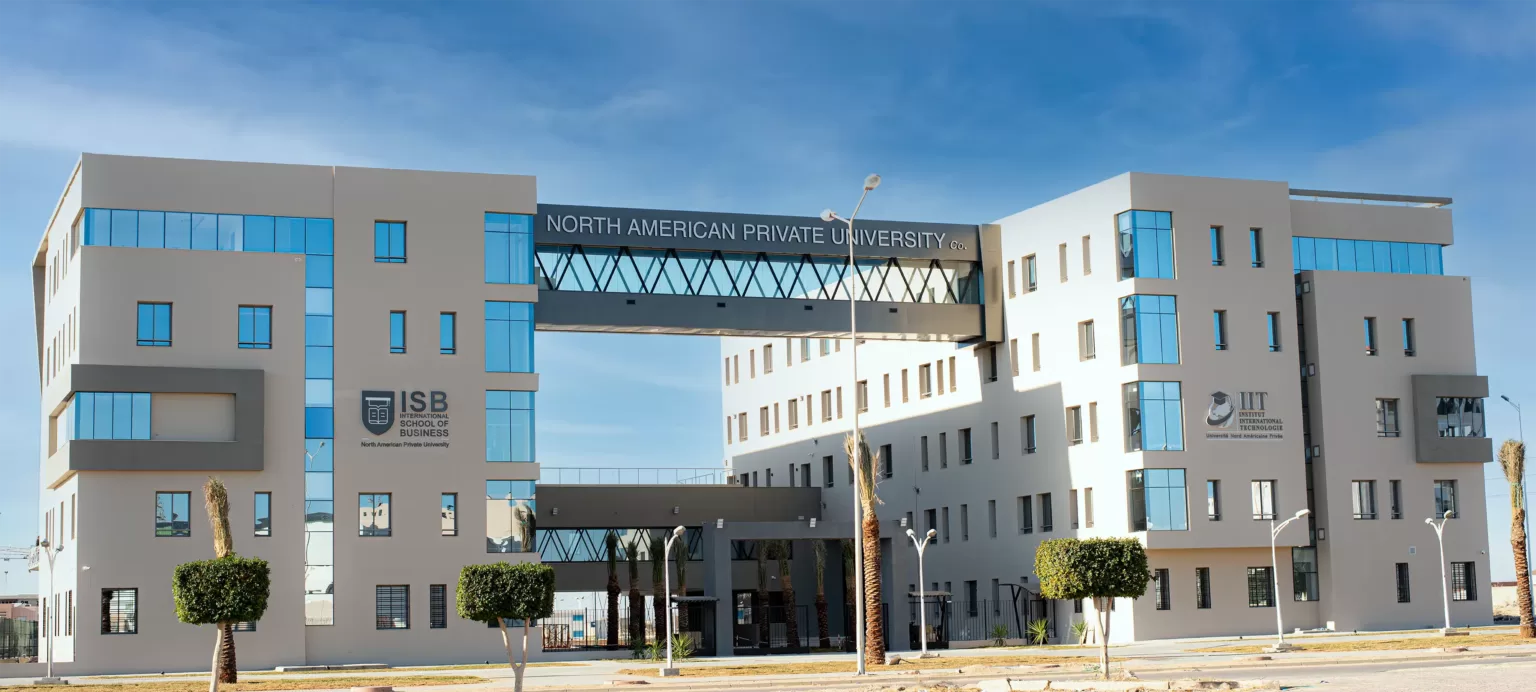
\includegraphics[width=0.9\textwidth]{../IIT_Sfax_Template/images/TemplateImages/Image-Exemple.jpg}
\caption{Login Page}
\end{figure}

The login screen includes:
\begin{itemize}
    \item IIT Logo
    \item Email/password form
    \item "Sign In" button with arrow icon
    \item Role-based redirect after login
\end{itemize}

%\subsection{Admin Dashboard}

\begin{figure}[H]
%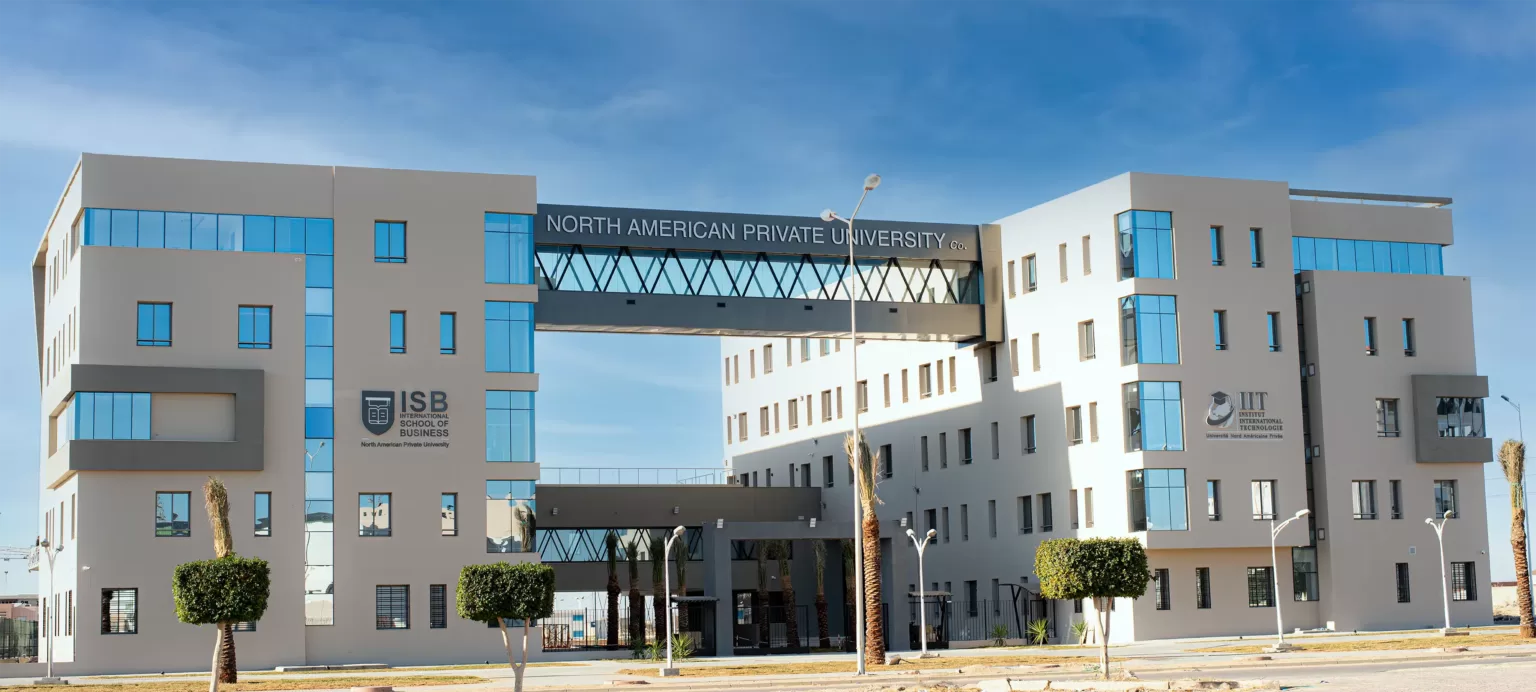
\includegraphics[width=0.9\textwidth]{../IIT_Sfax_Template/images/TemplateImages/Image-Exemple.jpg}
\caption{Admin Dashboard}
\end{figure}

%\subsection{User Management}

\begin{figure}[H]
%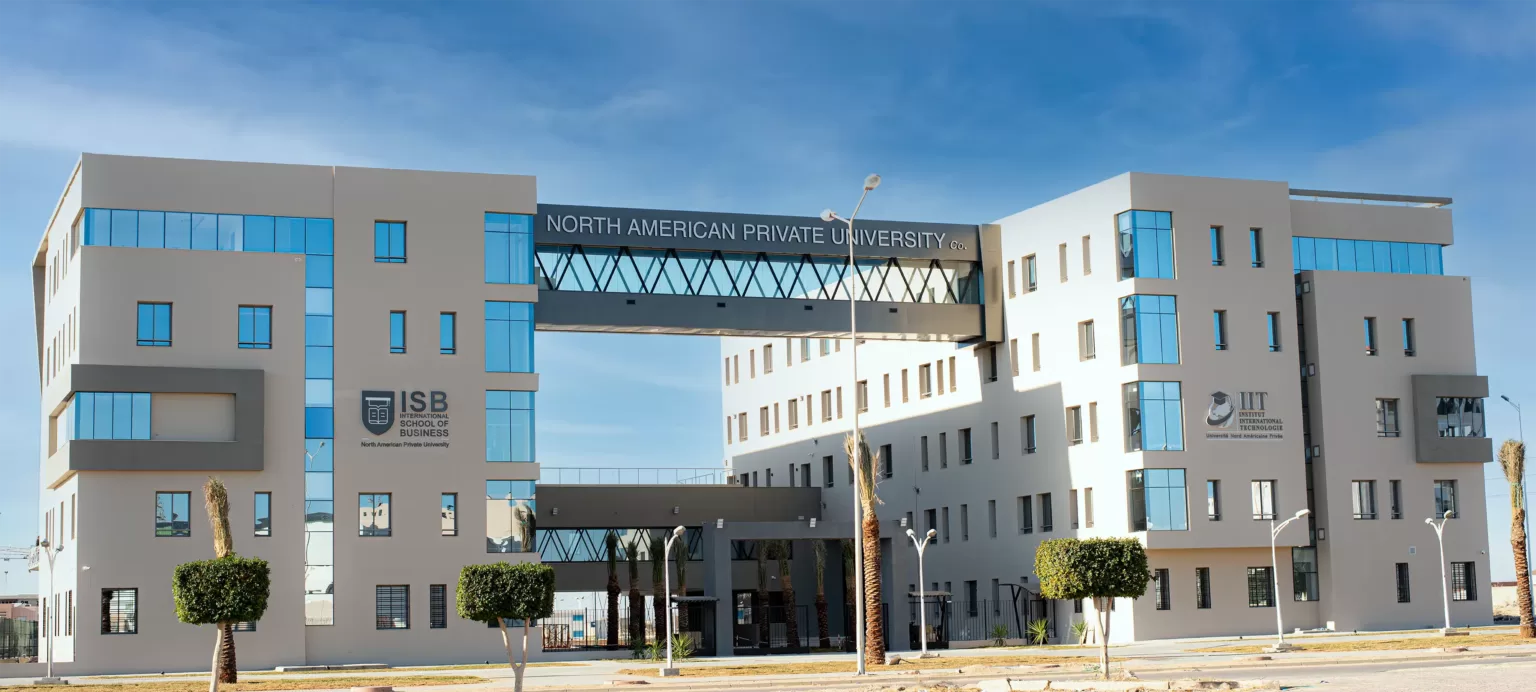
\includegraphics[width=0.9\textwidth]{../IIT_Sfax_Template/images/TemplateImages/Image-Exemple.jpg}
\caption{User Management Page}
\end{figure}

%\subsection{Supervisor Management}

\begin{figure}[H]
%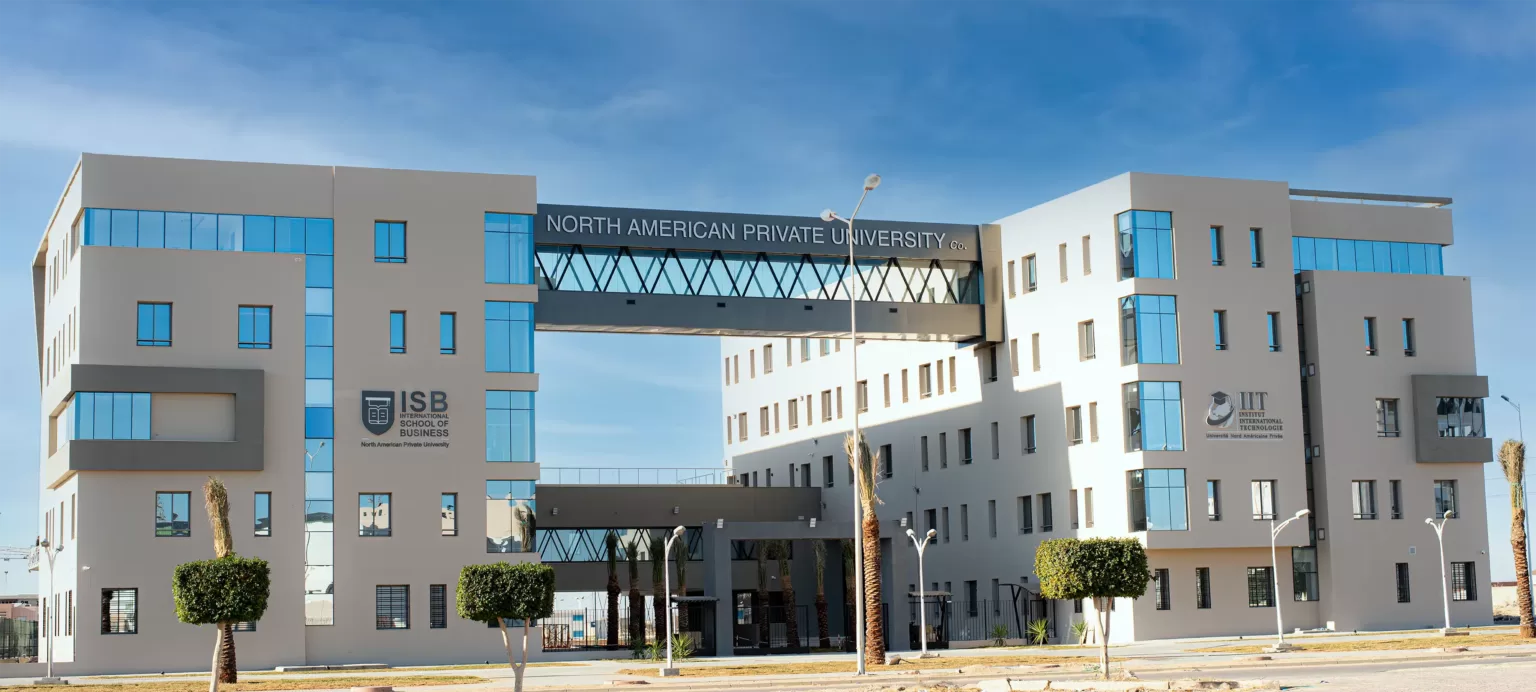
\includegraphics[width=0.9\textwidth]{../IIT_Sfax_Template/images/TemplateImages/Image-Exemple.jpg}
\caption{Supervisor Management Page}
\end{figure}

%\subsection{Quiz Interface}

\begin{figure}[H]
%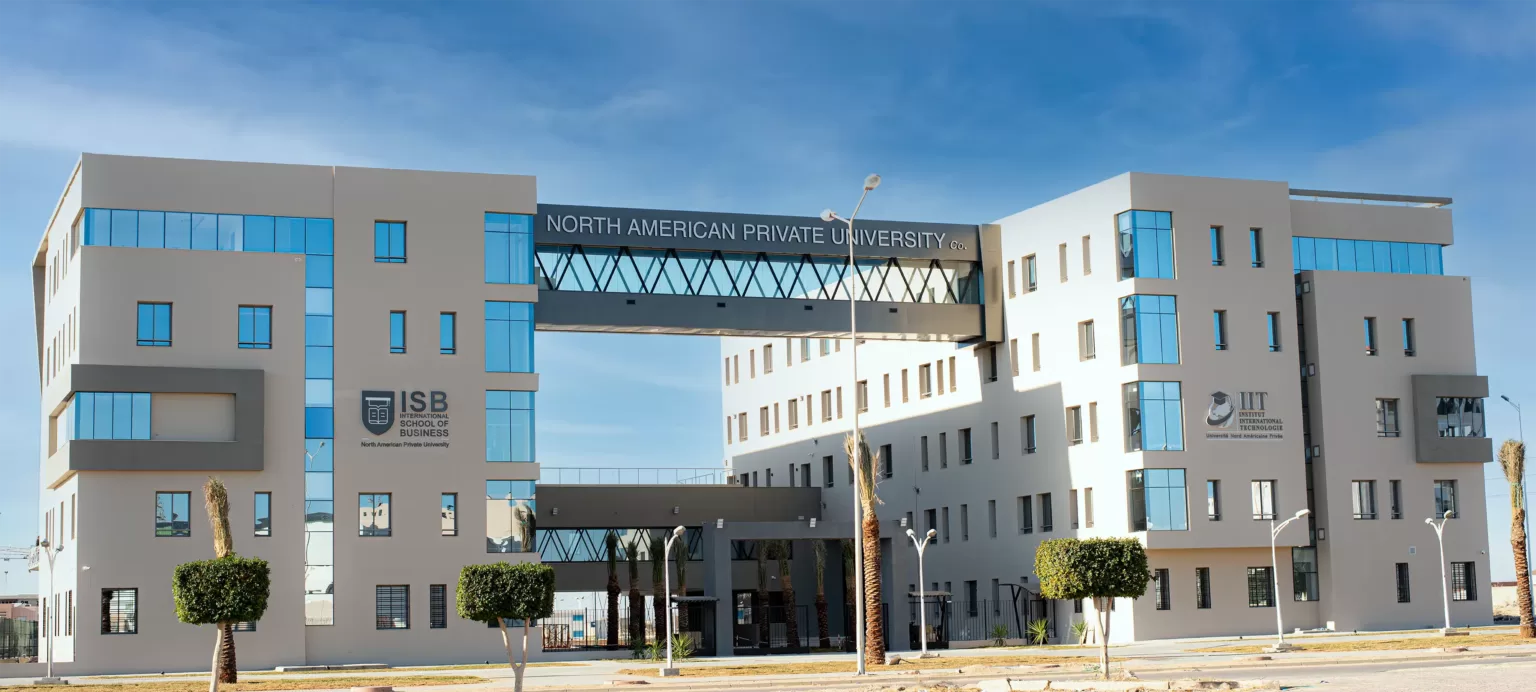
\includegraphics[width=0.9\textwidth]{../IIT_Sfax_Template/images/TemplateImages/Image-Exemple.jpg}
caption{Quiz Interface}
\end{figure}

The quiz interface includes:
\begin{itemize}
    \item 48-hour visible timer
    \item Multiple choice questions (A, B, C, D)
    \item Question navigation
    \item Automatic submission at end
    \item Immediate result with score
\end{itemize}

\pagebreak

%=======================================================================
% CHAPTER 6: CHALLENGES AND SOLUTIONS
% ============================================================================
\chapter{CHALLENGES AND SOLUTIONS}

\section{Technical Challenges}

\subsection{Challenge 1: Login/Logout Bug}
\textbf{Problem}: Login works first time, fails on subsequent attempts after logout.

\textbf{Solution}:
\begin{itemize}
    \item Implemented Nuclear Logout - clears all localStorage and sessionStorage
    \item Added useEffect in LoginPage to detect state change and redirect
    \item Used ref to track login attempt
    \item Role-based redirect: Admin/Manager → Dashboard, Receptionist → Reception Panel, Candidate → Quiz Interface
\end{itemize}

\begin{figure}[H]
%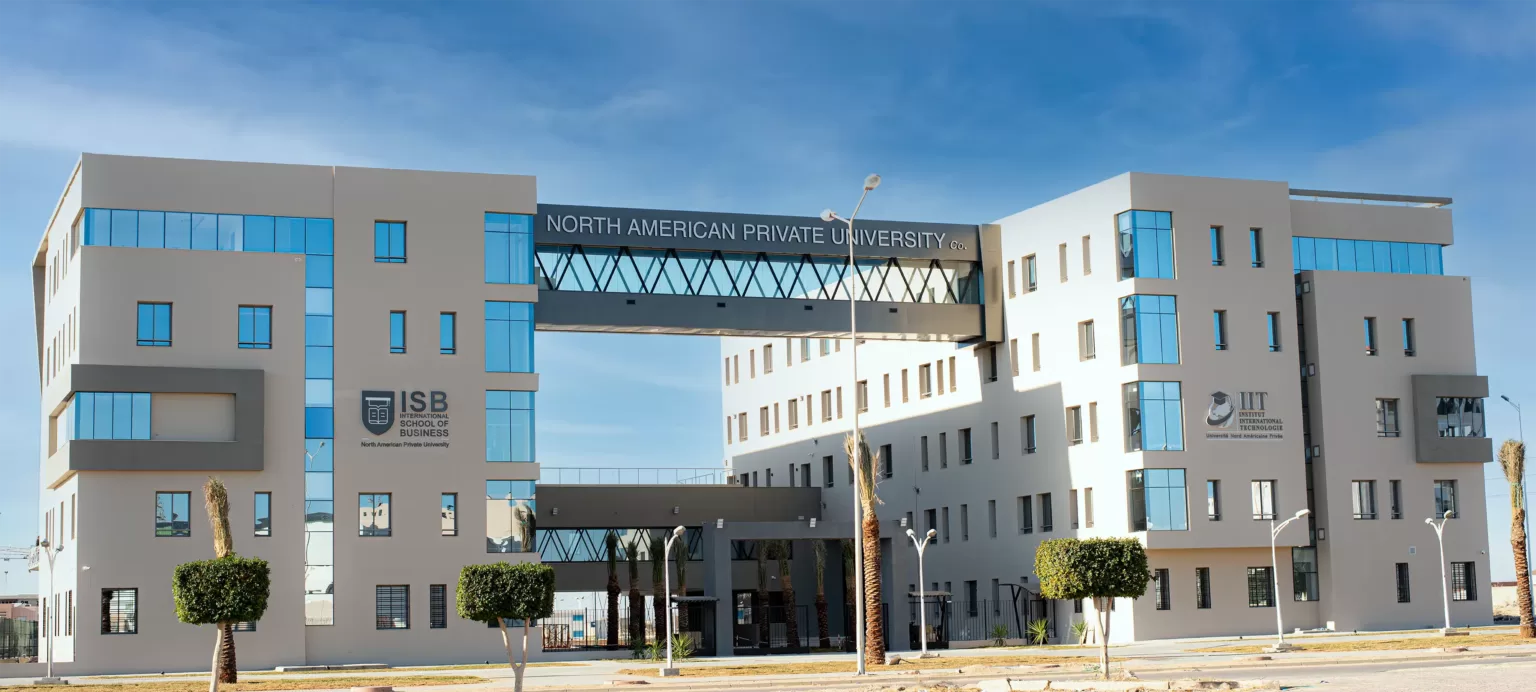
\includegraphics[width=0.9\textwidth]{../IIT_Sfax_Template/images/TemplateImages/Image-Exemple.jpg}
caption{Login Flow - Solution}
\end{figure}

\subsection{Challenge 2: Backend Not Running}
\textbf{Problem}: API calls fail when backend is down.

\textbf{Solution}: Added demo mode in axios.js with localStorage:
\begin{itemize}
    \item usersApi - stores in localStorage
    \item supervisorsApi - stores in localStorage
    \item authApi - checks stored users
    \item notificationsApi - returns empty
    \item dashboardApi - returns zeros
\end{itemize}

\subsection{Challenge 3: Secure Password Generation}
\textbf{Problem}: Need secure temporary passwords for new users.

\textbf{Solution}:
\begin{lstlisting}[language=JavaScript]
const generateSecurePassword = (length = 12) => {
  const charset = 'abcdefghijklmnopqrstuvwxyzABCDEFGHIJKLMNOPQRSTUVWXYZ0123456789!@#$%^&*';
  const array = new Uint32Array(length);
  crypto.getRandomValues(array);
  return Array.from(array, i => charset[i % charset.length]).join('');
};
\end{lstlisting}

\section{Business Challenges}

\subsection{Challenge 4: Quiz 48-Hour Limit}
\textbf{Problem}: Quiz must be completed within 48 hours.

\textbf{Solution}: Added QuizTimeLimitInterceptor in backend:
\begin{itemize}
    \item Stores startedAt timestamp
    \item Calculates expiresAt = startedAt + 48 hours
    \item Rejects submissions after expiry
    \item Sets score to 0 if time exceeded
\end{itemize}

\subsection{Challenge 5: Password Reset on First Login}
\textbf{Problem}: New users must change temporary password.

\textbf{Solution}:
\begin{itemize}
    \item Added mustChangePassword flag in User entity
    \item Login checks flag and redirects to /reset-password
    \item resetPassword() in AuthContext updates the flag
    \item After reset, redirects to appropriate panel
\end{itemize}

\pagebreak

%=======================================================================
% CHAPTER 7: CONCLUSION
% ============================================================================
\chapter{CONCLUSION}

\section{Project Summary}
The \textbf{Smart Internship \& Project Management System (SIPMS)} is a complete web application that allows:

\begin{enumerate}
    \item \textbf{Digitizing} the entire internship management process
    \item \textbf{Automating} technical evaluations by quiz
    \item \textbf{Integrating} artificial intelligence functionalities
    \item \textbf{Securing} access by JWT authentication and RBAC
    \item \textbf{Notifying} users automatically by email and in-app
    \item \textbf{Managing} users and supervisors with CRUD operations
    \item \textbf{Generating} secure temporary passwords
\end{enumerate}

\section{Results Obtained}

\begin{table}[H]
\centering
\begin{tabular}{|l|l|c|}
\hline
\textbf{Module} & \textbf{Functionality} & \textbf{Status} \\ \hline
Auth & JWT Connection & ✅ \\ \hline
Auth & Role-Based Redirect & ✅ \\ \hline
Auth & Password Reset & ✅ \\ \hline
Management & User CRUD (Demo Mode) & ✅ \\ \hline
Management & Supervisor CRUD (Demo Mode) & ✅ \\ \hline
Application & Online Submission & ✅ \\ \hline
Reception & Physical Files & ✅ \\ \hline
Quiz & Timed Quiz (48h) & ✅ \\ \hline
Quiz & Auto Evaluation & ✅ \\ \hline
AI & Project Ranking & ✅ \\ \hline
AI & Supervisor Matching & ✅ \\ \hline
Notifications & In-App + Email & ✅ \\ \hline
Dashboard & Statistics & ✅ \\ \hline
\end{tabular}
\caption{Results - Implemented Features}
\end{table}

\section{Future Improvements}
Several features can be added:

\begin{enumerate}
    \item \textbf{Video Interview}: Video conferencing integration
    \item \textbf{Calendar}: Interview scheduling
    \item \textbf{Reporting}: PDF report generation
    \item \textbf{Multi-lingual}: Arabic/English/French support
    \item \textbf{Mobile App}: Native mobile application
    \item \textbf{Public API}: For external integration
    \item \textbf{Real Backend}: Connect to real MySQL instead of demo mode
\end{enumerate}

\section{Lessons Learned}
This project allowed:
\begin{itemize}
    \item Mastering full-stack development with Spring Boot and React
    \item Understanding web security issues (JWT, RBAC)
    \item Implementing simple AI algorithms (TF-IDF, matching)
    \item Working with Tailwind CSS for responsive design
    \item Debugging complex state management issues
    \item Technically documenting a complete project
    \item Creating professional reports with LaTeX
\end{itemize}

\pagebreak

%=======================================================================
% APPENDICES
% ============================================================================
\appendix
\chapter{APPENDIX A: API Endpoints}

\section{Authentication}
\begin{itemize}
    \item POST /api/auth/login - User login
    \item POST /api/auth/register - User registration
    \item POST /api/auth/refresh - Token refresh
\end{itemize}

\section{Users (Admin)}
\begin{itemize}
    \item GET /api/users - List all users
    \item POST /api/users - Create user
    \item PUT /api/users/\{id\} - Update user
    \item DELETE /api/users/\{id\} - Delete user
    \item PATCH /api/users/\{id\}/toggle-active - Toggle status
\end{itemize}

\section{Supervisors}
\begin{itemize}
    \item GET /api/supervisors - List supervisors
    \item POST /api/supervisors - Create supervisor
    \item PUT /api/supervisors/\{id\} - Update supervisor
    \item DELETE /api/supervisors/\{id\} - Delete supervisor
\end{itemize}

\section{Applications}
\begin{itemize}
    \item GET /api/applications - List applications
    \item POST /api/applications - Submit application
    \item POST /api/applications/physical - Physical registration
    \item PATCH /api/applications/\{id\}/status - Update status
    \item PATCH /api/applications/\{id\}/assign-supervisor - Assign supervisor
\end{itemize}

\section{Quiz}
\begin{itemize}
    \item GET /api/quiz - List quizzes
    \item GET /api/quiz/\{id\} - Get quiz details
    \item POST /api/quiz/submit - Submit quiz answers
    \item GET /api/quiz/results - Get quiz results
\end{itemize}

\pagebreak

\chapter{APPENDIX B: Database Schema}

\section{Users Table}
\begin{table}[H]
\centering
\begin{tabular}{|l|l|l|}
\hline
\textbf{Column} & \textbf{Type} & \textbf{Description} \\ \hline
id & BIGINT & Primary key \\ \hline
first\_name & VARCHAR(100) & First name \\ \hline
last\_name & VARCHAR(100) & Last name \\ \hline
email & VARCHAR(255) & Unique email \\ \hline
password\_hash & VARCHAR(255) & Encrypted password \\ \hline
active & BOOLEAN & Active status \\ \hline
must\_change\_password & BOOLEAN & Password reset flag \\ \hline
created\_at & TIMESTAMP & Creation date \\ \hline
updated\_at & TIMESTAMP & Modification date \\ \hline
\end{tabular}
\end{table}

\section{Applications Table}
\begin{table}[H]
\centering
\begin{tabular}{|l|l|l|}
\hline
\textbf{Column} & \textbf{Type} & \textbf{Description} \\ \hline
id & BIGINT & Primary key \\ \hline
candidate\_id & BIGINT & Candidate reference \\ \hline
project\_id & BIGINT & Project reference \\ \hline
supervisor\_id & BIGINT & Supervisor reference \\ \hline
status & ENUM & Workflow status \\ \hline
intake\_method & ENUM & ONLINE/PHYSICAL \\ \hline
manager\_notes & TEXT & Decision notes \\ \hline
ai\_match\_score & DOUBLE & AI score \\ \hline
created\_at & TIMESTAMP & Creation date \\ \hline
\end{tabular}
\end{table}

\pagebreak

\chapter{APPENDIX C: User Manual}

\section{Admin User}
\begin{enumerate}
    \item Login with admin credentials (admin@sipms.com / Admin@123)
    \item Navigate to User Management to create new users
    \item System auto-generates secure passwords
    \item Navigate to Supervisor Management to add supervisors
    \item View dashboard for statistics
\end{enumerate}

\section{New User (Candidate/Receptionist)}
\begin{enumerate}
    \item Login with email and temporary password
    \item System redirects to /reset-password
    \item Enter new password
    \item System redirects to appropriate panel:
    \begin{itemize}
        \item Receptionist → /reception-panel
        \item Candidate → /quiz-interface
    \end{itemize}
\end{enumerate}

\section{Candidate User}
\begin{enumerate}
    \item Login and change temporary password
    \item Submit application with project idea
    \item Take assigned quiz within 48 hours
    \item View results and status
\end{enumerate}

\pagebreak

%=======================================================================
% REFERENCES
% ============================================================================
\chapter{REFERENCES}

\begin{thebibliography}{99}

bibitem{react} React Documentation. \textit{Facebook Inc.}, 2024. https://reactjs.org/

bibitem{spring} Spring Boot Documentation. \textit{VMWare Inc.}, 2024. https://spring.io/projects/spring-boot

bibitem{jwt} JWT Specification. \textit{Auth0 Inc.}, 2024. https://jwt.io/

bibitem{tailwind} Tailwind CSS Documentation. \textit{Tailwind Labs}, 2024. https://tailwindcss.com/

bibitem{mysql} MySQL Documentation. \textit{Oracle Corporation}, 2024. https://dev.mysql.com/

bibitem{hibernate} Hibernate ORM Documentation. \textit{Red Hat Inc.}, 2024. https://hibernate.org/orm/

bibitem{vite} Vite Documentation. \textit{Evan You}, 2024. https://vitejs.dev/

\end{thebibliography}

%=======================================================================
% END OF DOCUMENT
%=======================================================================
\end{document}